To evaluate the performance of the Monocular View Volume Registration (MVVR) method, both qualitative and quantitative types of experiment results are presented. In these experiments, the MVVR method was compared against the proposed FVR method. In some experiments, the Microsoft Life-Cam HD3000 passive camera was used capturing $640 \times 480$ images. In some comparisons, the ASUS Xtion PRO LIVE camera was used, but the MVVR method only made use of the information from the RGB frames. These images were processed and successive frames were used to generate depth maps. Each depth map was projected into volume sizes of $256^3$ for processing by the rest of the MVVR method (namely the FVR part). To generate the depth maps, a local 2D block matching method was used. Kernel sizes used in the correlation procedure were $3 \times 3$ in size with a search area size of $21 \times 21$. The sizes of the kernel, search area and volume sizes were all chosen empirically. \\


For the qualitative comparison RGB-D frames were captured of a scene using the ASUS Xtion PRO LIVE active camera, RGB-D information was fed into the FVR registration method whilst only RGB monocular data was fed into the MVVR algorithm. Figure 5 shows the qualitative comparison between the reconstruction generated via the FVR method (left) with the MVVR method (right) using the clock video stream. This video stream was captured by translating and rotating the camera slowly between frames. The depth maps computed by the block matching method are only an estimation of the true scene depth and therefore the projection is only relative to the
actual depth. However the 3D data in the registration is still spatially accurate relative to the different parts of the geometry within the scene. Comparing the noise levels between depth maps produced by block matching and RGB-D hardware from figure 2 we can
see how much more noise the monocular volume registration
method must tolerate in order to generate the output. \\


\begin{figure}[!htb]
        \centering
        \begin{subfigure}[b]{1.5in}
                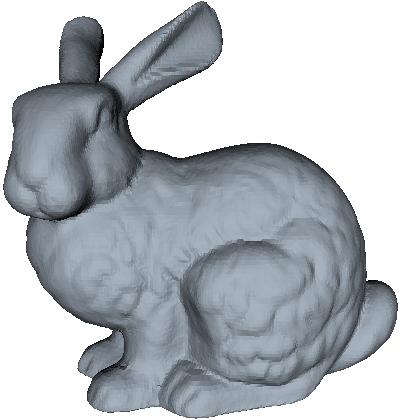
\includegraphics[width=1.5in]{images/ch2/bunny}
                \caption{original}
                \label{fig:bunnyOrigAA2}
        \end{subfigure}%
        \begin{subfigure}[b]{1.5in}
                
\includegraphics[width=1.5in]{images/methodology/FVR/xaxis}
                \caption{X-Axis Projection Map Domain}
                \label{fig:xaxPMDOM}
        \end{subfigure}
        \begin{subfigure}[b]{1.5in}
                
\includegraphics[width=1.5in]{images/methodology/FVR/yaxis}
                \caption{Y-Axis Projection Map Domain}
                \label{fig:yaxPMDOM}
        \end{subfigure}%
        \begin{subfigure}[b]{1.5in}
                
\includegraphics[width=1.5in]{images/methodology/FVR/zaxis}
                \caption{Z-Axis Projection Map Domain}
                \label{fig:zaxPMDOM}
        \end{subfigure}
        \caption{The Projection Map Transform.}
       \label{fig:pmtExample}
\end{figure}

Figure 6 shows results from a similar experiment, this
time using the Boxes video stream. As with the previous
scene, this stream was captured by moving the camera over the scene so that the environment is scanned in. The
monocular algorithm is once again able to generate a dense
3D model of the environment, with the exception that
sections of continuous texture, which cannot be picked up by
block matching, are filtered out.



\begin{figure}[!htb]
        \centering
        \begin{subfigure}[b]{1.5in}
                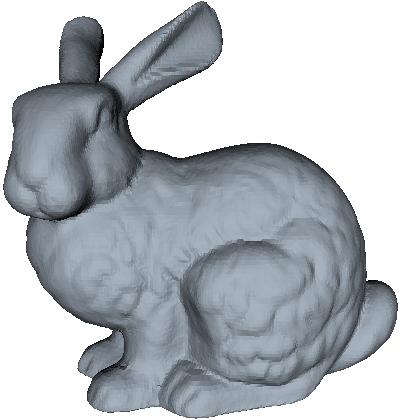
\includegraphics[width=1.5in]{images/ch2/bunny}
                \caption{original}
                \label{fig:bunnyOrigAA2}
        \end{subfigure}%
        \begin{subfigure}[b]{1.5in}
                
\includegraphics[width=1.5in]{images/methodology/FVR/xaxis}
                \caption{X-Axis Projection Map Domain}
                \label{fig:xaxPMDOM}
        \end{subfigure}
        \begin{subfigure}[b]{1.5in}
                
\includegraphics[width=1.5in]{images/methodology/FVR/yaxis}
                \caption{Y-Axis Projection Map Domain}
                \label{fig:yaxPMDOM}
        \end{subfigure}%
        \begin{subfigure}[b]{1.5in}
                
\includegraphics[width=1.5in]{images/methodology/FVR/zaxis}
                \caption{Z-Axis Projection Map Domain}
                \label{fig:zaxPMDOM}
        \end{subfigure}
        \caption{The Projection Map Transform.}
       \label{fig:pmtExample}
\end{figure}

These experiments show that with almost identical
qualitative performance to the RGB-D volume registration
method and without performing any feature matching, the
MVVR method is able to register dense depth data and
produce results comparable to the RGB-D volume
registration method despite the noise prevalent in the block
matching depth estimates. \\
In order to assess the method quantitatively, we captured
frames as the camera was moved in 5, 10 and 15 cm
increments and registered information between frames. Then
estimated camera movements were compared to actual
movements and graphed in figure 7.

Movement
5cm
10cm
15cm
RGB-D VR Error
0cm
0cm
0cm
MVVR Error
0cm
0cm
27cm


Figure 7 shows that unlike the results reported in [1], the
RGB-D VR method was able to register with 100% accuracy
for frames with 15cm of camera movement. In the previous
work it was reported as 2.8cm error. However, as shown here
this can vary depending on the data used for testing. Using
the same data, whilst ignoring inconsistent and noisy depth
maps, the MVVR method was able to register up to 10cm of
camera movement without fault. With movements of 10cm
and frame rates of 30 frames per second, this equates to
speeds of roughly 10 km per hour which is about twice as
fast as walking speed.